\documentclass[11pt,a4paper]{article}
\usepackage[margin=2.2cm]{geometry}
\usepackage[T1]{fontenc}
\usepackage{lmodern}
\usepackage{amsmath,amssymb}
\usepackage{graphicx}
\usepackage{booktabs}
\usepackage{caption}
\usepackage{subcaption}
\usepackage{xcolor}
\usepackage{tikz}
\usetikzlibrary{arrows.meta,positioning,shapes.geometric}
\usepackage[colorlinks=true,linkcolor=blue!50!black,urlcolor=blue!50!black,citecolor=blue!50!black]{hyperref}

\graphicspath{{figures/}}
\captionsetup{font=small,labelfont=bf}
\newcommand{\us}{\,\mu\mathrm{s}}
\newcommand{\Dinf}{D_\infty}
\newcommand{\Tinf}{T_\infty}

\title{Spectral and Bispectral Neutron Multiplicity Counting\\for Plutonium Mass Assay\\[4pt]
\large A simulation study with OpenMC}
\author{Michel Saliba}
\date{20 October 2026}

\begin{document}
\maketitle

\begin{abstract}
\noindent
Passive neutron multiplicity counting finds the mass of a plutonium item from the time
correlations between detected neutrons. The standard instrument is the shift register,
which counts neutrons in time gates and needs calibrated gate fractions $f_d$ and $f_t$.
This report tests a frequency-domain alternative. Doubles are read from the 3-bank
\emph{cross power spectral density} and Triples from the 3-bank \emph{cross-bispectrum}.
In these spectra the uncorrelated background cancels by construction, and no gate
fractions are needed. We simulate a 300\,g Pu metal sphere in a 3-bank He-3 well counter
with OpenMC, build 300\,s list-mode pulse trains, and analyse them with both methods.
Over repeated measurements the bispectrum is unbiased ($+0.8\pm1.1\%$ on the mass) but noisier
($\approx9$\,g per 300\,s run). A shift register calibrated with a Cf-252 source is precise
($\approx2$\,g) but biased by $+4.5\%$, and by $+5.3\%$ for a moderated item, because the
calibration source has no fission-chain timing. The best result comes from a hybrid in which
the bispectrum calibrates the shift-register gate fraction: about 3\,g RMS error on 300\,g.
\end{abstract}

\tableofcontents

%==========================================================================
\section{Neutron multiplicity counting in brief}
%==========================================================================
Pu-240 (and the other even isotopes) fissions spontaneously and emits $\nu$ neutrons
\emph{at the same time}, with $\nu$ distributed by $P(\nu)$. Other neutrons are emitted
one at a time by $(\alpha,n)$ reactions on light elements. Some neutrons cause further
fissions inside the item (self-multiplication $M$). A well counter moderates the neutrons
in polyethylene and captures them in He-3. The capture of each neutron is delayed by a
random die-away time, about $\tau\approx50\us$.

The detector therefore sees a stream of pulses with a Poisson background of uncorrelated
neutrons, plus small \emph{bursts} of correlated neutrons from each fission chain. Three
rates summarise this stream:
\begin{itemize}
  \item \textbf{Singles} $S$: all detected neutrons per second.
  \item \textbf{Doubles} $\Dinf$: correlated \emph{pairs} per second (pairs from the same fission chain).
  \item \textbf{Triples} $\Tinf$: correlated \emph{triplets} per second.
\end{itemize}
The Böhnel point model links these three rates to three unknowns: the spontaneous-fission
rate $F$ (proportional to the Pu-240 effective mass), $M$, and
$\alpha=$ ($\alpha,n$ neutrons)/(SF neutrons):
\begin{align}
S &= F\varepsilon M\nu_{s1}(1+\alpha), \label{eq:S}\\
\Dinf &= \tfrac{1}{2}F\varepsilon^2M^2\Big[\nu_{s2}+\tfrac{M-1}{\nu_{i1}-1}\nu_{s1}(1+\alpha)\nu_{i2}\Big],\\
\Tinf &= \tfrac{1}{6}F\varepsilon^3M^3\Big[\nu_{s3}+\tfrac{M-1}{\nu_{i1}-1}\big(3\nu_{s2}\nu_{i2}+\nu_{s1}(1+\alpha)\nu_{i3}\big)
        +3\big(\tfrac{M-1}{\nu_{i1}-1}\big)^2\nu_{s1}(1+\alpha)\nu_{i2}^2\Big].
\end{align}
Here $\varepsilon$ is the detection efficiency, and $\nu_{sk}$, $\nu_{ik}$ are the factorial
moments of the spontaneous and induced fission multiplicity distributions. Eliminating $F$
and $\alpha$ gives a cubic equation in $M$. Its physical root ($M\ge1$) gives $M$, then
$F$, then $\alpha$. The Pu mass is $m_{\text{Pu}}=F/(473.5\,\text{s}^{-1}\text{g}^{-1})/f_{240}$.

\textbf{The whole problem is measuring $\Dinf$ and $\Tinf$ accurately.} This report compares
two ways of doing so.

%==========================================================================
\section{Simulation set-up}
%==========================================================================
\subsection{What OpenMC is}
OpenMC is an open-source Monte Carlo neutron and photon transport code, developed at MIT
and Argonne. It tracks individual particles through a 3D constructive-solid-geometry model
using continuous-energy nuclear data (here ENDF/B-VIII.1). It supports fixed-source
problems. Its \texttt{collision\_track} feature writes every selected collision to an HDF5
file, with position, time, reaction, nuclide and the history ID. This event-by-event output
is what a list-mode multiplicity study needs.

\subsection{Model}
\begin{table}[h]
\centering\small
\begin{tabular}{@{}lp{0.78\linewidth}@{}}
\toprule
Item & Value \\
\midrule
Pu sphere & 300\,g, $\rho=15.8$\,g/cm$^3$, $r=1.654$\,cm; 94\,wt\% Pu-239, 6\,wt\% Pu-240 ($m_{\text{eff}}=18$\,g) \\
SF rate & $F=473.5\times18=8523$\,fissions/s;\ $\alpha=0.50$ \\
Cavity & void cylinder, $r=4$\,cm, $|z|<4$\,cm (end plugs close the top and bottom) \\
Detector body & cylinder $r=20$\,cm, $|z|<20$\,cm; HDPE ($0.96$\,g/cm$^3$, S($\alpha,\beta$) \texttt{c\_H\_in\_CH2}) \\
Absorber & He-3 mixed homogeneously, $1.2\times10^{-5}$\,atoms/(b\,cm) \\
Banks & 3 azimuthal $120^\circ$ sectors X, Y, Z (cells 101--103) \\
Source & uniform in the sphere, isotropic, Pu-240 SF Watt spectrum ($a=0.795$\,MeV, $b=4.689$\,MeV$^{-1}$) \\
\bottomrule
\end{tabular}
\caption{Model parameters (\texttt{config/assay\_config.json}).}
\end{table}

\begin{figure}[h]
\centering
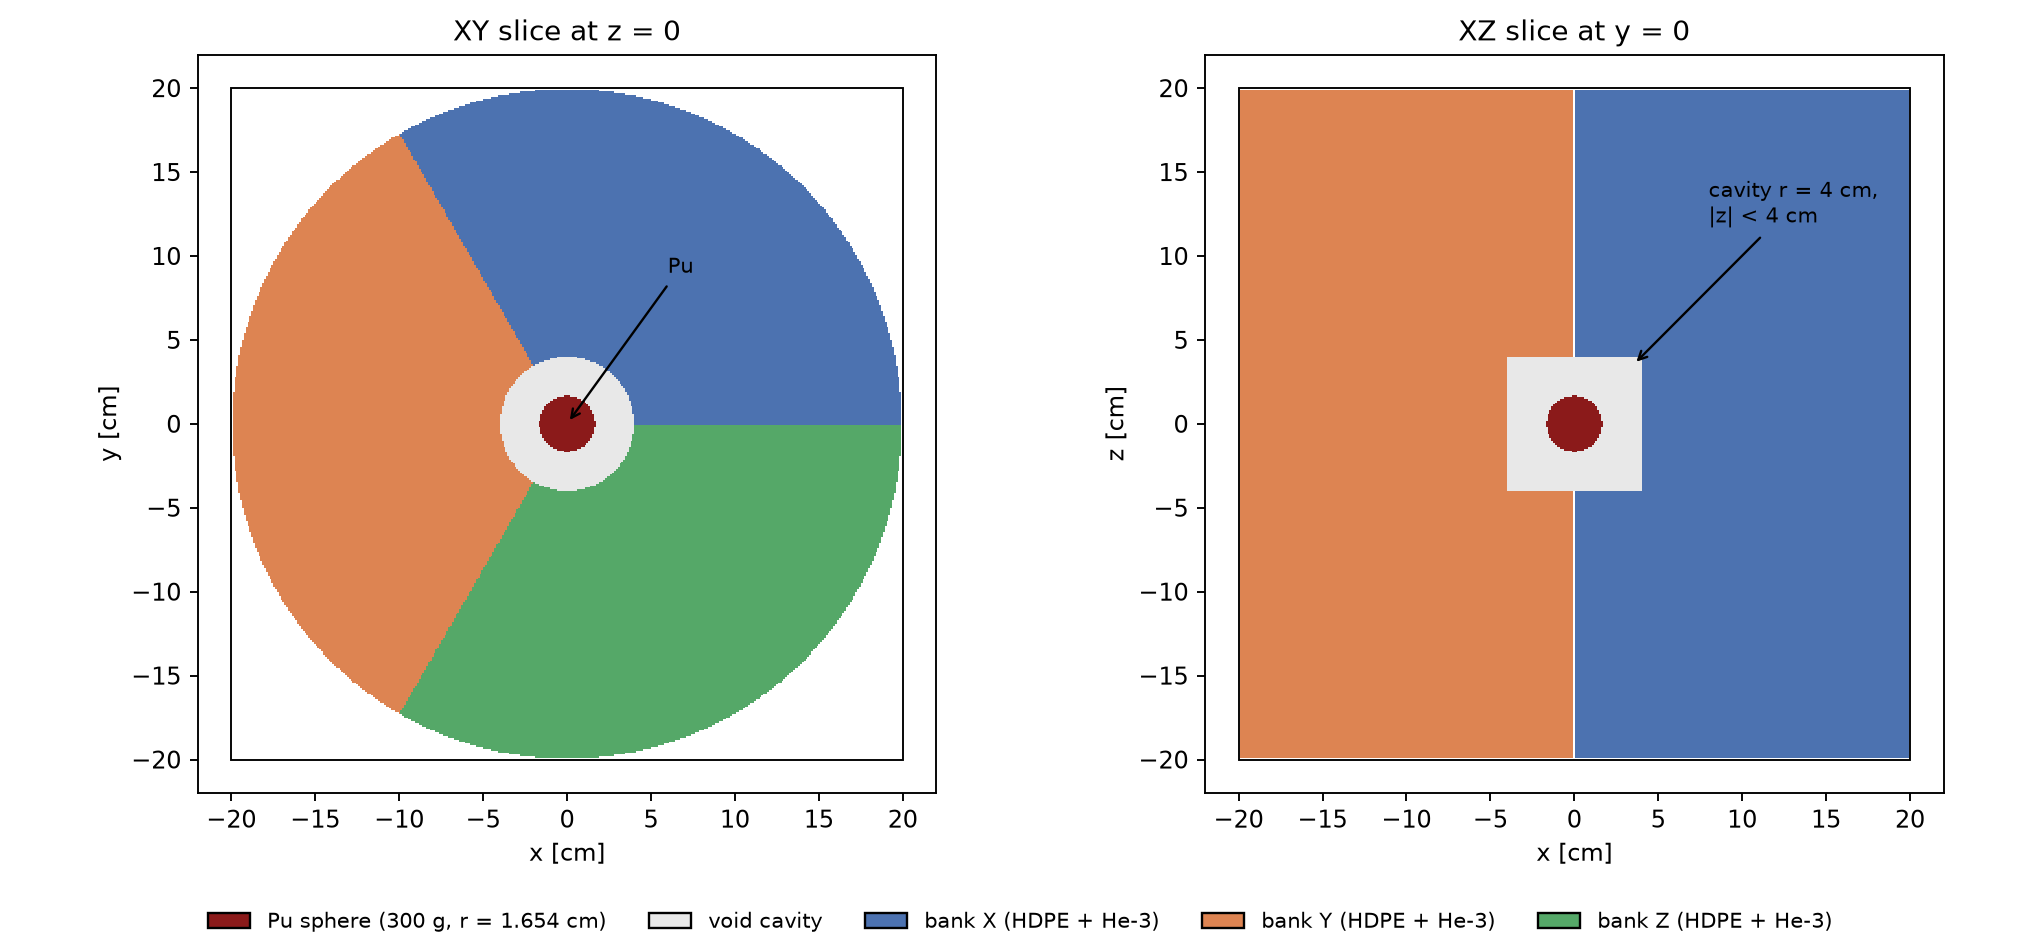
\includegraphics[width=0.78\linewidth]{geometry_slices.png}\hfill
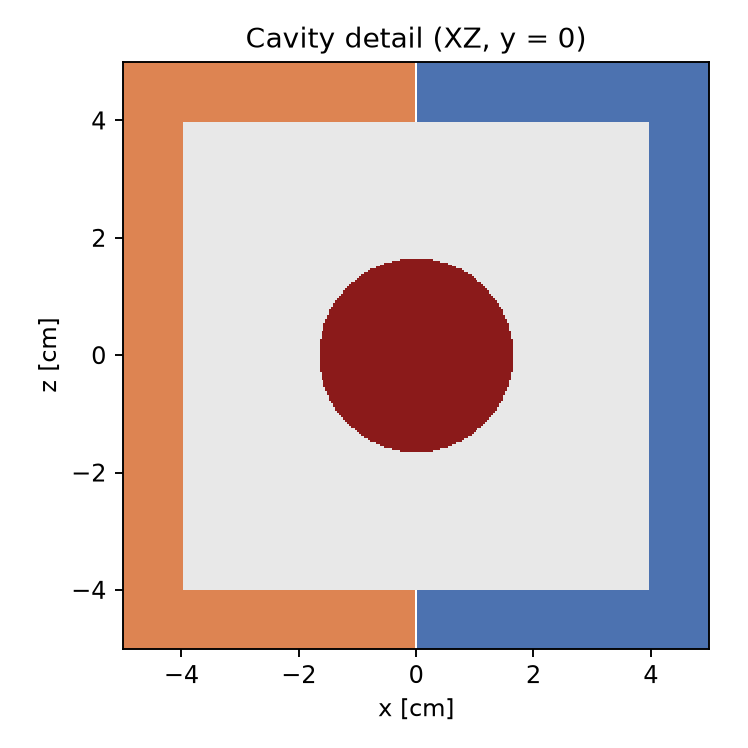
\includegraphics[width=0.21\linewidth]{geometry_zoom.png}
\caption{OpenMC geometry, rasterised from the model's own cell definitions. Left: XY slice
showing the three $120^\circ$ detector banks around the cavity. Middle: XZ slice; the end
plugs enclose the sphere almost $4\pi$. Right: cavity detail.}
\label{fig:geom}
\end{figure}

\begin{figure}[h]
\centering
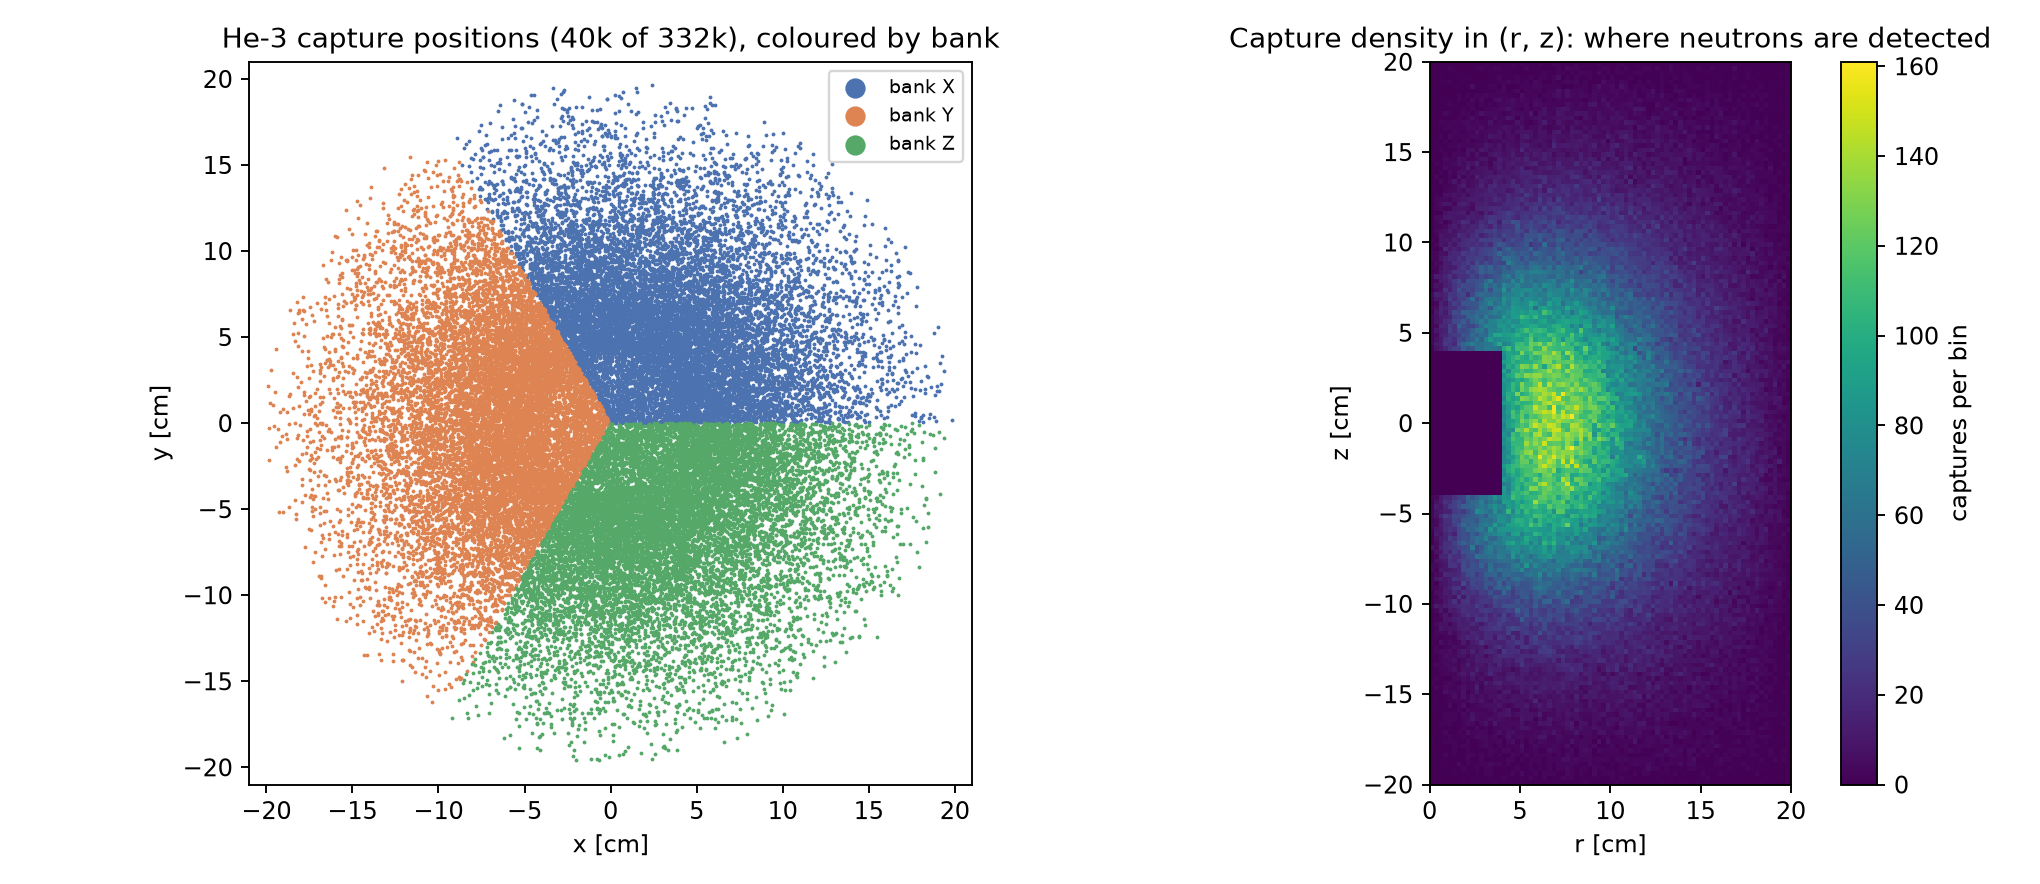
\includegraphics[width=0.9\linewidth]{capture_maps.png}
\caption{Where neutrons are detected (400k source histories). Left: He-3 capture positions
coloured by bank. Right: capture density in $(r,z)$. Most captures occur 3--10\,cm into
the polyethylene, after thermalisation.}
\label{fig:capt}
\end{figure}

\subsection{OpenMC features used}
\begin{itemize}
  \item \texttt{run\_mode = 'fixed source'}, \texttt{survival\_biasing = False} (analog captures), one batch of 400\,000 histories.
  \item \texttt{collision\_track}: cells 101--103, nuclide He-3, reaction MT\,101 (absorption). Each record is one detection, with its \texttt{time}, position \texttt{r} (which gives the bank) and \texttt{parent\_id} (the source history).
  \item \texttt{surf\_source\_write} on the sphere surface: the net outward crossings per source neutron give the leakage multiplication $M_{\text{MC}}$.
  \item Default physics otherwise. OpenMC treats fission \emph{implicitly} in fixed-source mode: fission neutrons are banked as an expected value at each Pu collision. The mean multiplication is right, but the spread of neutrons per induced fission is not. We keep this as an approximation and calibrate \emph{effective} induced-fission moments $\nu_{i2}=4.85$, $\nu_{i3}=0.22$ from the transport output. Both methods use them, so the comparison is fair.
\end{itemize}

\subsection{From single histories to a measurement}
OpenMC gives the response to \emph{one} source neutron starting at $t=0$: a list of
(capture delay, bank) pairs. A 300\,s measurement is then assembled in Python:
\begin{enumerate}
  \item Draw $N_{\text{SF}}\sim\text{Poisson}(FT)$ fission times, uniform in $[0,T]$, with $\nu\sim P(\nu)$ (Pu-240).
  \item Draw $(\alpha,n)$ emission times at rate $F\nu_{s1}\alpha$, one neutron each.
  \item Give every emitted neutron a random OpenMC history, and shift its captures by the birth time.
  \item Merge everything and sort by time. The result is 6.85 million pulses with time stamps and bank labels.
\end{enumerate}
Because every step is known, the \emph{exact} expected rates follow from the factorial
moments of the per-history detected counts ($m_1,m_2,m_3$). We use them as ground truth:
$S=22854$, $\Dinf=17404$, $\Tinf=13835$\,s$^{-1}$.

\begin{figure}[h]
\centering
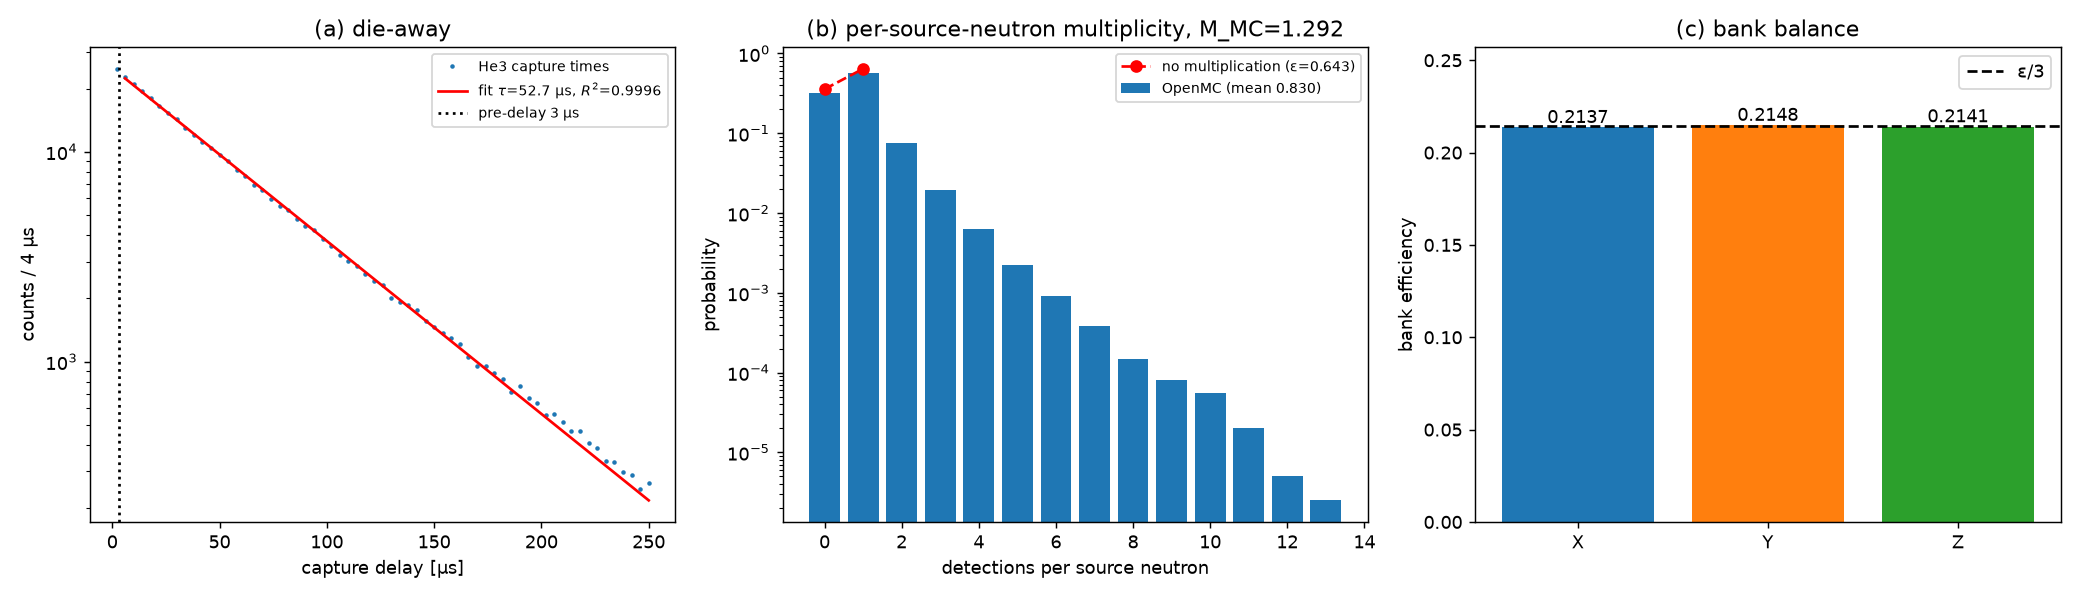
\includegraphics[width=\linewidth]{step_01_geometry_and_die_away.png}
\caption{Transport results. (a) He-3 capture-time distribution: $\tau=52.7\us$, $R^2=0.9996$.
(b) Detected counts per source neutron. The tail beyond 1 comes from induced fission ($M_{\text{MC}}=1.292$).
(c) Bank balance: $\varepsilon=0.643$, banks equal within 0.3\%.}
\end{figure}

\begin{figure}[h]
\centering
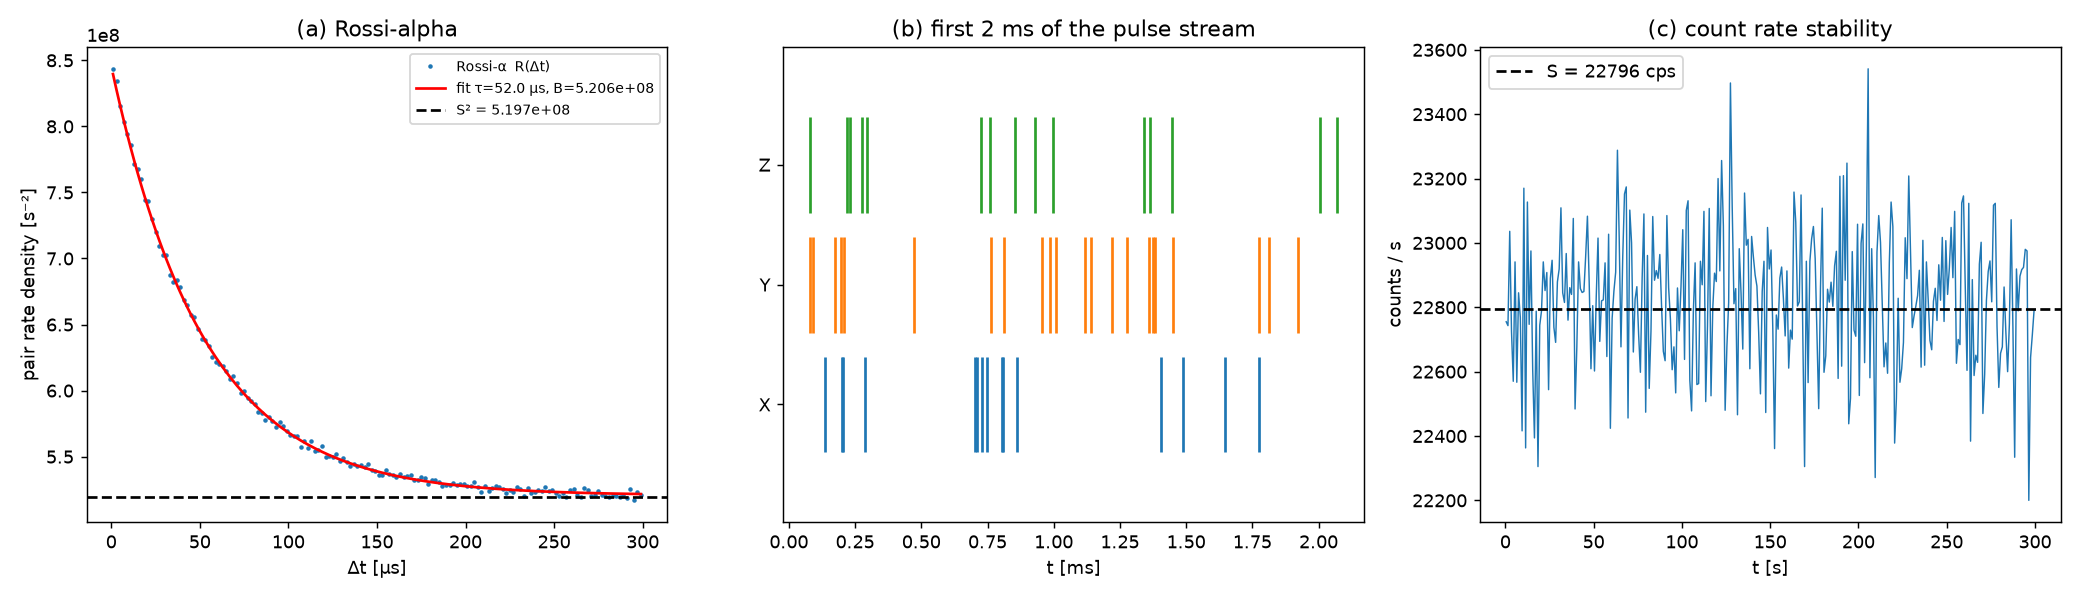
\includegraphics[width=\linewidth]{step_02_rossi_alpha_and_pulse_stream.png}
\caption{Synthetic pulse train. (a) Rossi-alpha distribution: correlated excess over the
$S^2$ baseline, decaying with $\tau\approx52\us$. (b) First 2\,ms of the stream per bank.
(c) Count rate is stable over 300\,s.}
\end{figure}

%==========================================================================
\section{Legacy method: the shift register}
%==========================================================================
Every pulse opens two gates of width $G=64\us$:
\begin{itemize}
  \item an \textbf{R+A} gate just after a pre-delay $P=3\us$: real (correlated) + accidental counts;
  \item an \textbf{A} gate after a long delay $L=2000\us$, when the correlation has died away: accidentals only (8 gates averaged).
\end{itemize}
Counting how many pulses fall in each gate gives the histograms $f(n)$ and $b(n)$. Their
reduced factorial moments give
\begin{equation}
D=S(f_1-b_1),\qquad T=S\big[(f_2-b_2)-b_1(f_1-b_1)\big].
\end{equation}
These are \emph{gated} rates. Only the fraction of correlated neutrons that falls inside the
gate is counted:
\begin{equation}
\Dinf=D/f_d,\qquad \Tinf=T/f_t,\qquad f_d=e^{-P/\tau}\big(1-e^{-G/\tau}\big),\ f_t\approx f_d^2 .
\end{equation}
We use empirical $f_d=0.657$, $f_t=0.434$, taken from the simulated die-away profile with
the neutrons assumed independent. This is the weak point. $f_t$ depends on the detailed
time structure of the fission chain, and in practice it comes from a calibration source.

\begin{figure}[h]
\centering
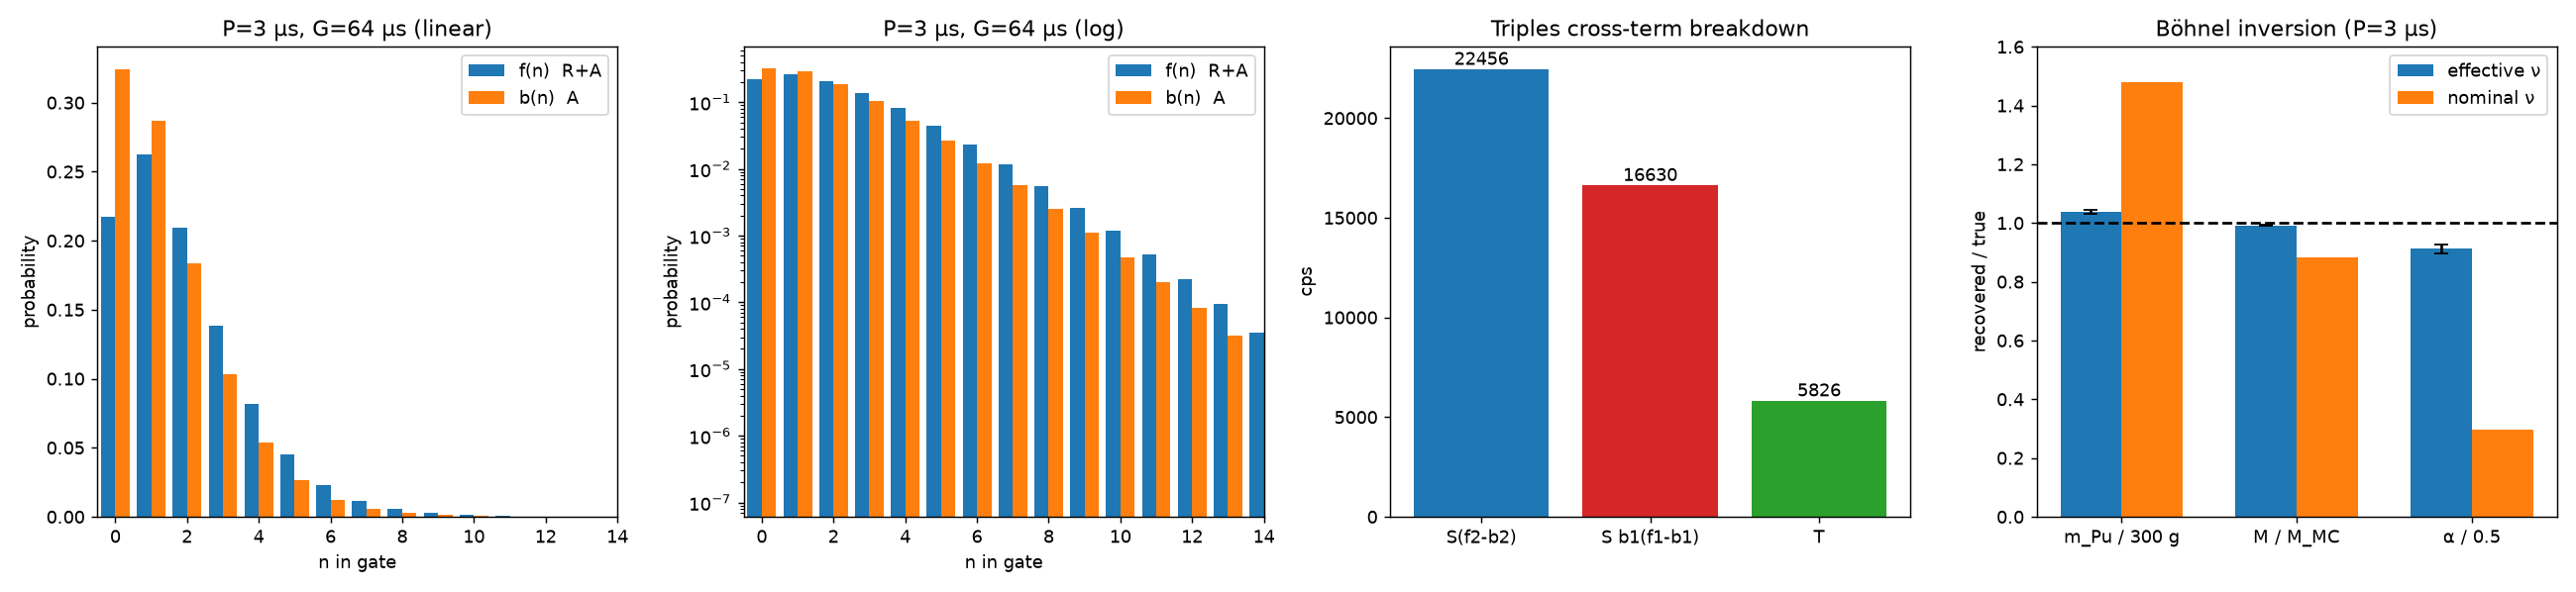
\includegraphics[width=\linewidth]{step_03_shift_register_histograms_and_inversion.png}
\caption{Shift register ($P=3\us$). Left: R+A and A histograms. Third panel: the accidental
cross-term $S\,b_1(f_1-b_1)$ is about three times larger than the final Triples, so $\Tinf$
is a small difference of large numbers. Right: inversion with the effective moments (blue)
and with the nominal Pu-239 moments (orange, +48\% mass, caused by the OpenMC
implicit-fission approximation).}
\end{figure}

\paragraph{Method 2A: DFT deconvolution of the histograms.} The R+A distribution is the
accidental distribution convolved with the distribution $p(k)$ of true correlated partners:
$f=p*b$. A Fourier transform turns the convolution into a product, so
$p=\text{IFFT}\big(\tilde f/\tilde b\big)$. Then $\Dinf=S\,r_1/f_d$ and
$\Tinf=S\,r_2/f_t$ with $r_1=\sum k\,p(k)$ and $r_2=\sum\binom{k}{2}p(k)$. The cross-term
disappears automatically. The results are identical to the shift register's, as they must
be, but the method still needs $f_d$ and $f_t$.

\begin{figure}[h]
\centering
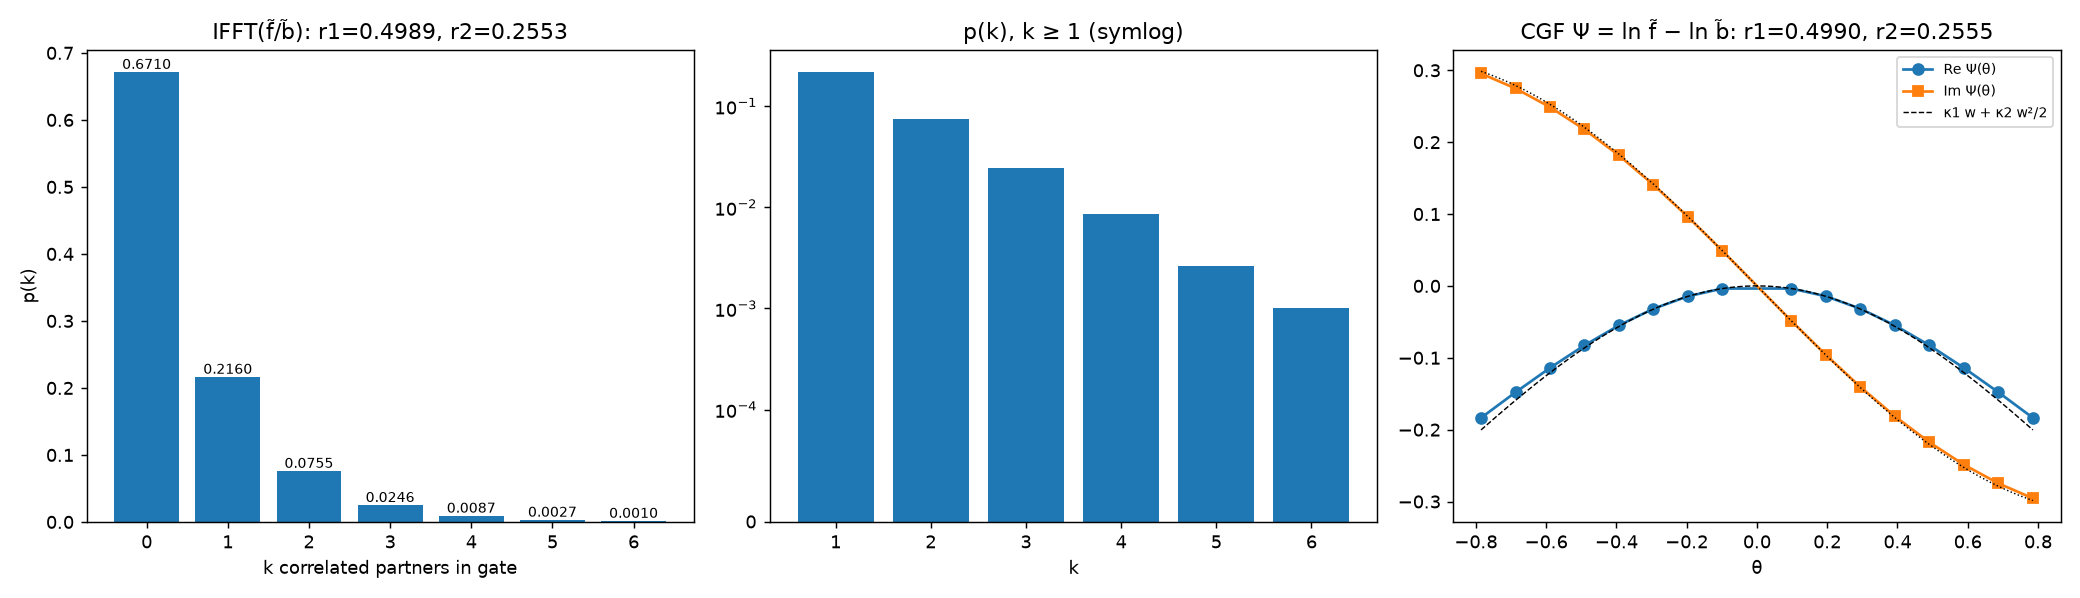
\includegraphics[width=\linewidth]{step_04a_dft_deconvolved_pk.png}
\caption{Method 2A. The deconvolved partner distribution $p(k)$, and the cumulant
generating function $\Psi=\ln\tilde f-\ln\tilde b$, whose low-order terms give the same $r_1$, $r_2$.}
\end{figure}

%==========================================================================
\section{New method: cross-spectrum and cross-bispectrum}
%==========================================================================
\subsection{Idea}
Instead of gates, look at the pulse train as a signal. Bin each bank into $\Delta t=2\us$
bins, giving $x(t)$, $y(t)$, $z(t)$. Cut the data into segments of $T_{\text{seg}}=16.4$\,ms
(18\,310 segments) and Fourier-transform each segment ($X(f)$, $Y(f)$, $Z(f)$). A correlated
burst born at time $t_0$ adds a phase $e^{-i\omega t_0}$ to every neutron it produces. In a
product of spectra in which the phases cancel, the burst survives averaging. Uncorrelated
neutrons average to zero. The detector die-away enters only through its transfer function
$h(\omega)$. For an exponential die-away $h(\omega)=1/(1+i\omega\tau)$, and in general
$h(0)=1$. This is the key point: \textbf{at zero frequency the die-away shape drops out}, so
no gate fraction is needed.

\subsection{Doubles from the cross power spectrum}
The power spectrum of the total signal is
\begin{equation}
S_{ss}(f)=\frac{\langle|X+Y+Z|^2\rangle}{T_{\text{seg}}}=S+2\Dinf|h(\omega)|^2 .
\end{equation}
The white floor is $S$, and the low-frequency plateau above it is $2\Dinf$. The
\textbf{cross}-PSD between different banks removes the floor, because one neutron can only
be in one bank:
\begin{equation}
S_{\text{cross}}(f)=\frac{\text{Re}\langle X^*Y+Y^*Z+Z^*X\rangle}{T_{\text{seg}}}
=2\Dinf\,|h(\omega)|^2\sum_{i<j}p_ip_j ,
\end{equation}
with $p_i$ the bank detection fractions ($\sum_{i<j}p_ip_j=1/3$ for equal banks).

\subsection{Triples from the cross-bispectrum}
The bispectrum is the next order. It multiplies three spectra whose frequencies add to zero:
\begin{equation}
B_{xyz}(f_1,f_2)=\frac{1}{T_{\text{seg}}}\text{Re}\Big\langle\overline{X(f_1)\,Y(f_2)\,Z^*(f_1+f_2)}\Big\rangle ,
\end{equation}
where the bar means an average over the 6 assignments of banks to the three slots. For a
triplet born at $t_0$, the phases $e^{-i\omega_1t_0}e^{-i\omega_2t_0}e^{+i(\omega_1+\omega_2)t_0}$
cancel. This gives
\begin{equation}
\frac{B_{xyz}(f_1,f_2)}{p_Xp_Yp_Z}=6\,\Tinf\;\text{Re}\big[h(\omega_1)\,h(\omega_2)\,h^*(\omega_1+\omega_2)\big].
\end{equation}
\textbf{Singles and Doubles vanish identically}: a single neutron hits one bank and a pair
at most two, but the product needs a neutron in each of the three banks. Only true triplets
(or larger bursts) contribute. The background subtraction that dominates the shift-register
Triples ($S\,b_1(f_1-b_1)$) is simply not there.

\subsection{How the method is applied}
\begin{center}
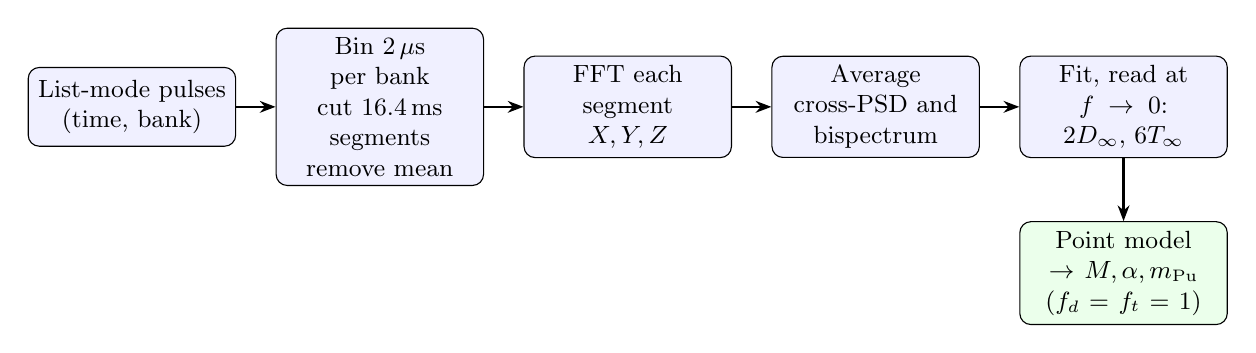
\begin{tikzpicture}[node distance=4mm and 5mm, every node/.style={font=\small},
  box/.style={draw,rounded corners,fill=blue!6,align=center,minimum height=10mm,text width=24mm},
  arr/.style={-{Stealth[length=2mm]},thick}]
\node[box] (a) {List-mode pulses\\(time, bank)};
\node[box,right=of a] (b) {Bin 2\,$\mu$s per bank\\cut 16.4\,ms segments\\remove mean};
\node[box,right=of b] (c) {FFT each\\segment\\$X,Y,Z$};
\node[box,right=of c] (d) {Average\\cross-PSD and\\bispectrum};
\node[box,right=of d] (e) {Fit, read at\\$f\to0$:\\$2\Dinf$, $6\Tinf$};
\node[box,below=8mm of e,fill=green!8] (f) {Point model\\$\to M,\alpha,m_{\text{Pu}}$\\($f_d=f_t=1$)};
\foreach \i/\j in {a/b,b/c,c/d,d/e,e/f} \draw[arr] (\i)--(\j);
\end{tikzpicture}
\end{center}
\begin{enumerate}
  \item Bin and segment the pulse train. Subtract each segment's mean count, so the
        uncorrelated DC terms cannot leak into the products.
  \item Accumulate the cross-PSD for $0<f\le100$\,kHz and the bispectrum on the grid
        $f_1\in(0,10]$\,kHz, $f_2\in[-10,10]$\,kHz ($163\times326$ points).
  \item Fit the spectra with a two-component die-away kernel
        $h(\omega)=\frac{1-w}{1+i\omega\tau_1}+\frac{w}{1+i\omega\tau_2}$ and read the
        zero-frequency amplitudes. The bispectrum gets its own free kernel.
  \item Insert $S$ (counted), $\Dinf$ and $\Tinf$ into the point model with $f_d=f_t=1$.
  \item Statistical errors come from the scatter over 10 independent time blocks.
\end{enumerate}

The two-component kernel matters. The real chain timing is not a pure exponential, because
some neutrons return from the moderator and cause a delayed thermal fission in the Pu.
With the single exponential $1/(1+i\omega\tau)$, the fits extrapolate to values that are too
low: $\Dinf=17116$ ($-1.7\%$) and $\Tinf=13191$ ($-4.7\%$). With the flexible kernel the
zero-frequency values agree with the truth.

\paragraph{Check on a toy signal.} Before the OpenMC data, the analysis was run on a
synthetic 3-bank stream with known rates and a $45\us$ exponential die-away. It gave
$\Dinf=7730$ (true 7800) and $\Tinf=2690$ (true 2700). The cross-PSD floor came out
$-1.1\pm4.3$, consistent with zero.

\begin{figure}[h]
\centering
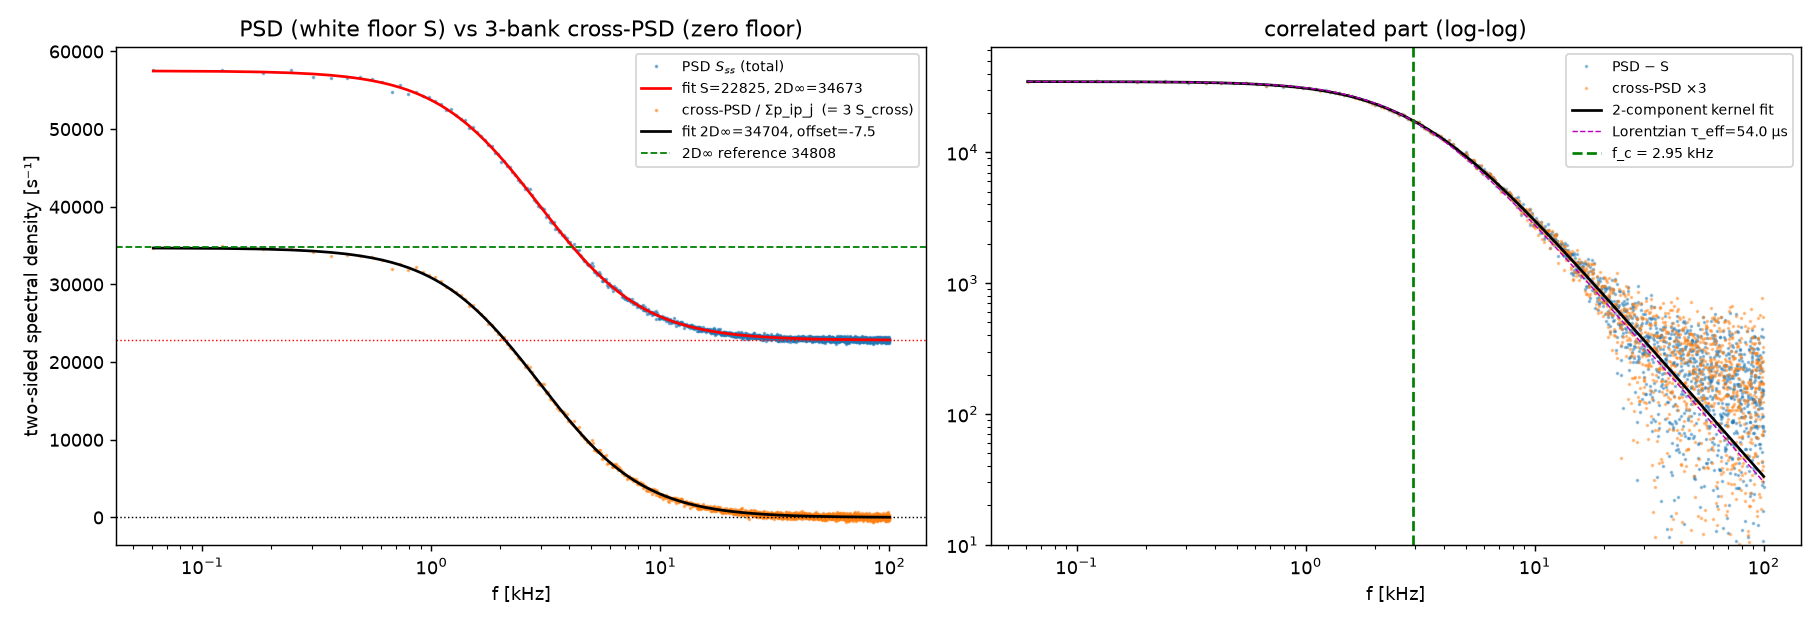
\includegraphics[width=\linewidth]{step_04b_psd_vs_cross_psd.png}
\caption{Doubles. Left: the total PSD sits on a white floor $S=22825$\,s$^{-1}$, while the
3-bank cross-PSD falls to zero (fitted offset $-7.5\pm4.9$). Both plateaus give
$2\Dinf\approx34\,700$, against the reference 34\,808. Right: the correlated part on a log
scale; corner frequency $f_c\approx3$\,kHz.}
\end{figure}

\begin{figure}[h]
\centering
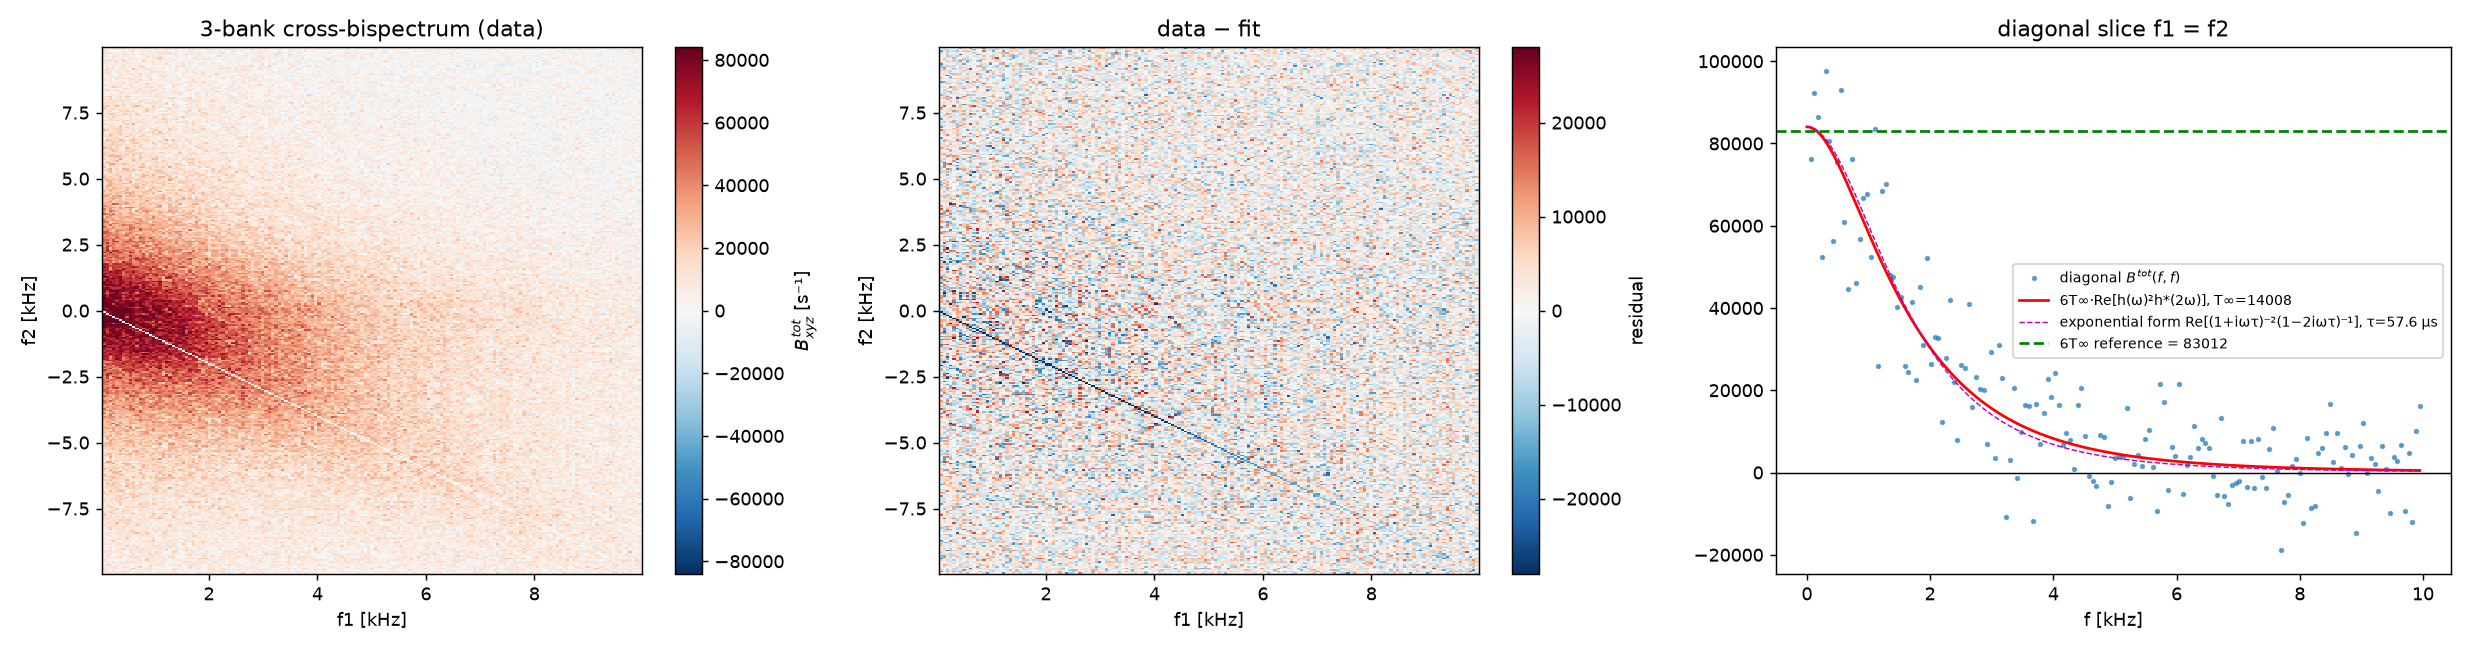
\includegraphics[width=\linewidth]{step_04c_cross_bispectrum_2d_and_diagonal.png}
\caption{Triples. Left: measured 3-bank cross-bispectrum $B^{\text{tot}}=B_{xyz}/(p_Xp_Yp_Z)$.
The signal sits near the origin and decays above a few kHz. The line $f_1+f_2=0$ is excluded
(zero after mean removal). Middle: residual after the fit, which is noise only. Right: the
diagonal slice $f_1=f_2$. The fitted curve reaches $6\Tinf$ at $f\to0$, close to the
reference (dashed).}
\end{figure}

%==========================================================================
\section{Results}
%==========================================================================
\begin{table}[h]
\centering\small
\setlength{\tabcolsep}{4pt}
\begin{tabular}{@{}lcccc@{}}
\toprule
Quantity & Ground truth & Shift register & 2A DFT & \textbf{New: cross-PSD + bispectrum} \\
\midrule
$S$ (s$^{-1}$)       & 22854 & $22822\pm12$ & $22822\pm12$ & $22822\pm12$ \\
$\Dinf$ (s$^{-1}$)   & 17404 & $17341\pm40$ ($-0.4\%$) & same & $17352\pm75$ ($-0.3\%$) \\
$\Tinf$ (s$^{-1}$)   & 13835 & $13421\pm78$ ($\mathbf{-3.0\%}$) & same & $14008\pm532$ ($+1.2\%$) \\
$M$                  & 1.292 & $1.281\pm0.002$ & same & $1.299\pm0.014$ \\
$\alpha$             & 0.50  & $0.456\pm0.008$ & same & $0.53\pm0.08$ \\
$m_{\text{eff}}$ (g) & 18.00 & $18.68\pm0.12$ & same & $17.5\pm0.8$ \\
$m_{\text{Pu}}$ (g)  & \textbf{300} & $\mathbf{311.3\pm2.0}$ ($+3.8\%$) & same & $\mathbf{291\pm14}$ ($-2.9\%$) \\
\bottomrule
\end{tabular}
\caption{Comparison for one 300\,s measurement. Errors are $1\sigma$ statistical.}
\label{tab:res}
\end{table}

\begin{figure}[h]
\centering
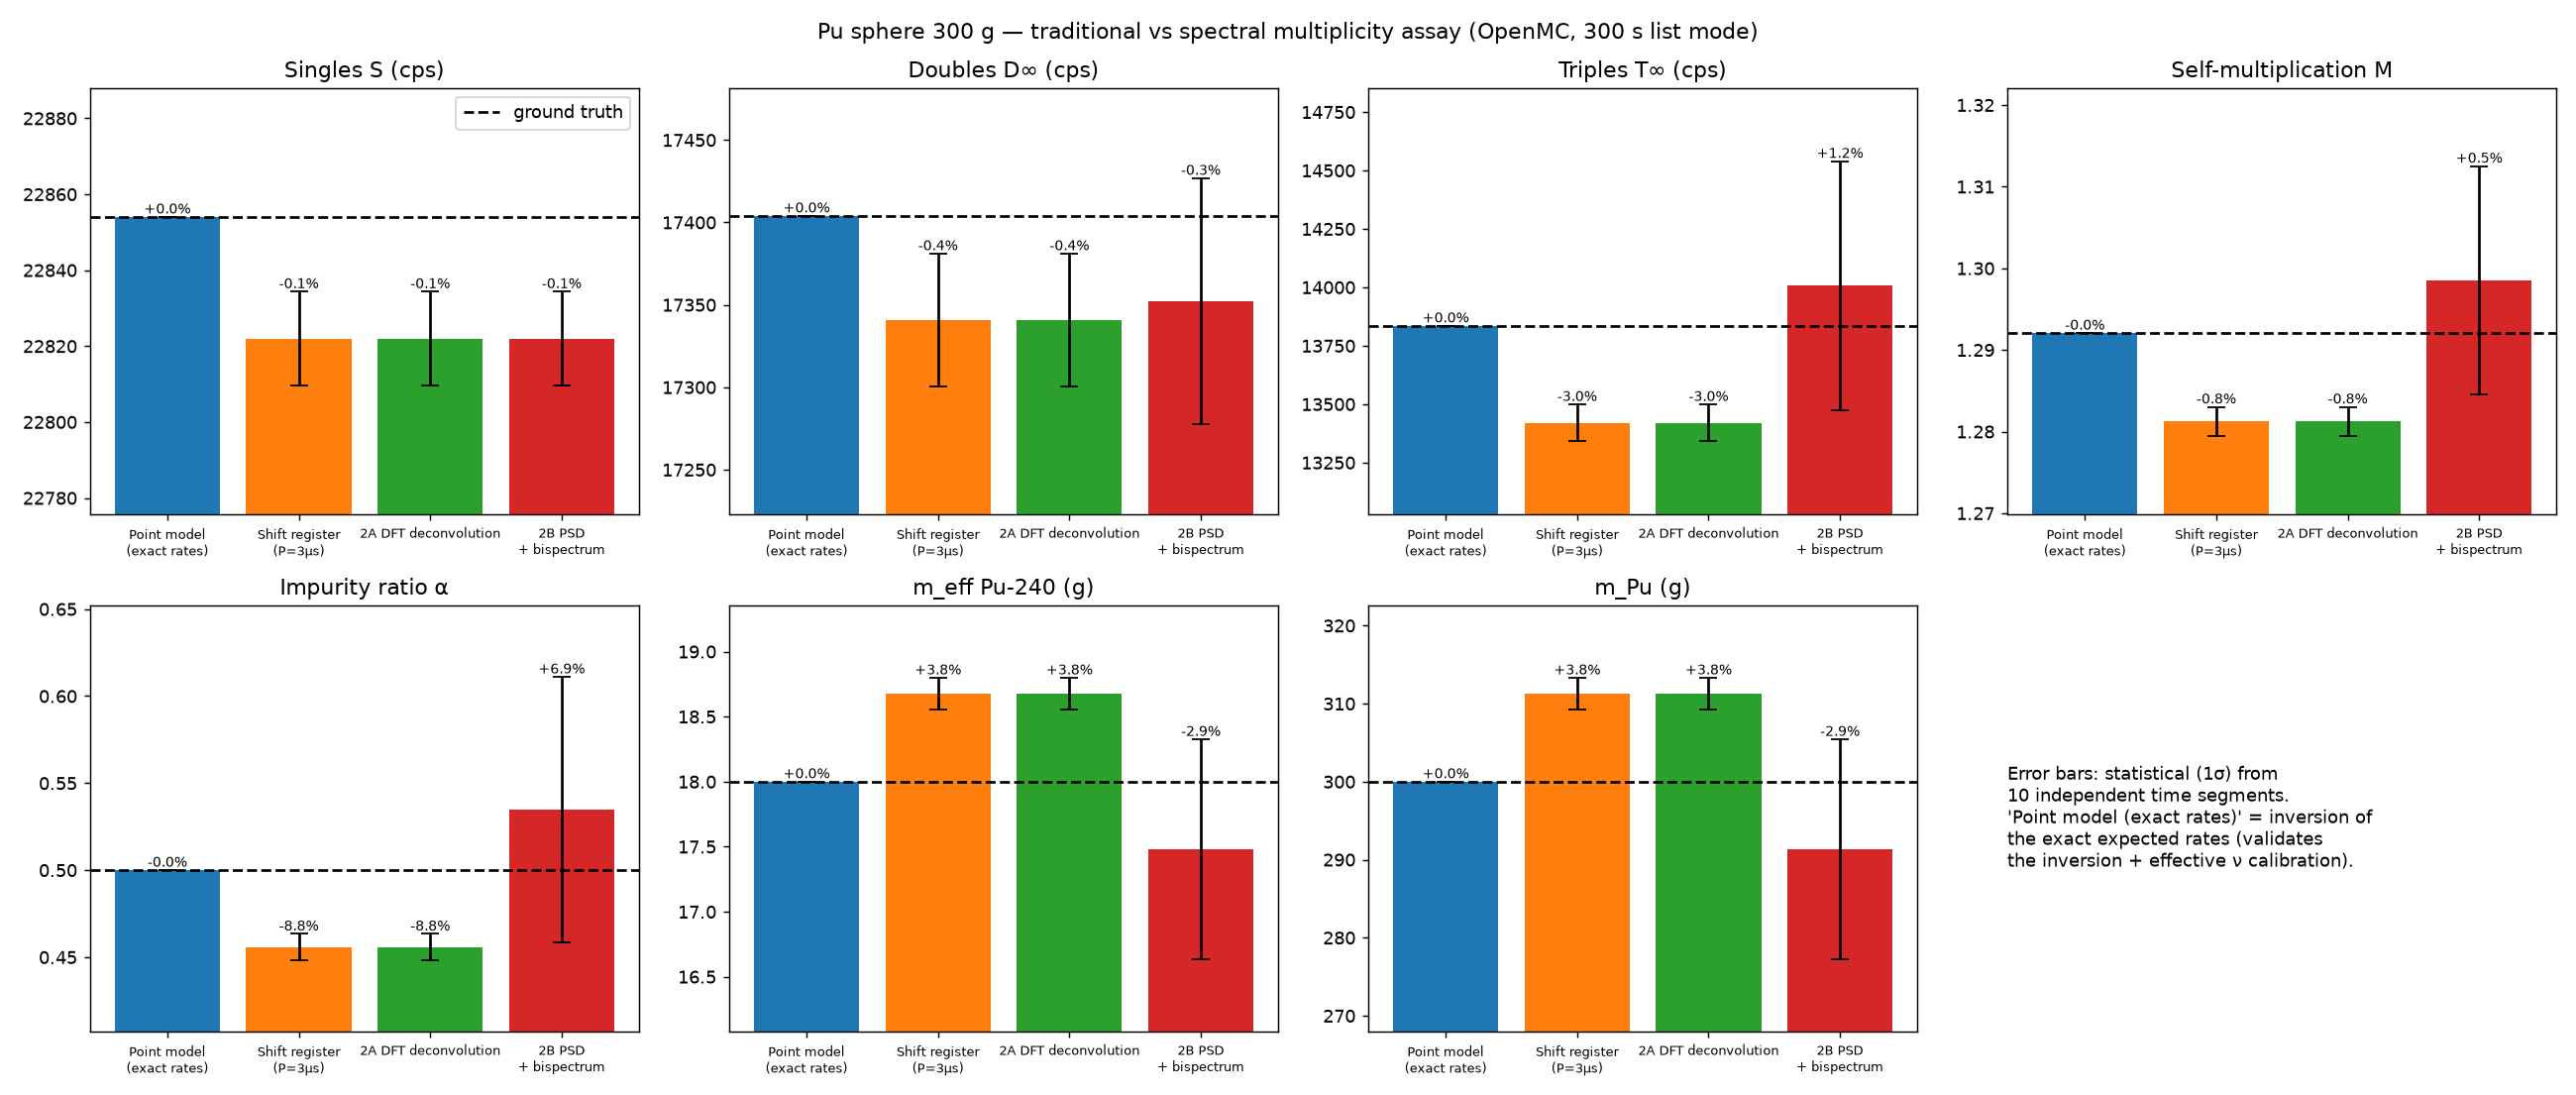
\includegraphics[width=\linewidth]{step_05_master_comparison.png}
\caption{Recovered quantities against ground truth (dashed). ``Point model (exact rates)''
inverts the exact expected rates and returns exactly 300\,g, which validates the inversion
and the effective-moment calibration.}
\end{figure}

%==========================================================================
\section{Why use the bispectrum? The case and its limits}
\label{sec:case}
%==========================================================================
\subsection{Arguments for}
\begin{enumerate}
  \item \textbf{No gate fractions.} The shift register converts gated counts to rates with
        $f_d$ and $f_t$. These depend on the die-away \emph{and} on the time structure
        inside a fission chain. The spectral rates are read at $f\to0$, where $h(0)=1$ for
        any die-away shape. The kernel is fitted on every measurement, so the method
        calibrates itself.
  \item \textbf{Background cancels by construction.} The cross-PSD has no Singles floor.
        The 3-bank bispectrum has neither a Singles nor a Doubles term. The shift-register
        Triples instead come from a subtraction whose cross-term $S\,b_1(f_1-b_1)$ is about
        three times larger than the result.
  \item \textbf{Diagnostic information.} The fitted kernel shows the real time structure of
        the detected chains, for example a slow component from neutrons that return to the
        item. A gate count cannot show this.
  \item \textbf{Observed accuracy.} In this study the bispectrum $\Tinf$ is $+1.2\%$ from
        truth (within $1\sigma$). The shift-register $\Tinf$ is $-3.0\%$ (about $5\sigma$).
\end{enumerate}

\subsection{Arguments against (so far)}
\begin{enumerate}
  \item \textbf{Precision.} The bispectrum $\Tinf$ is about 7 times noisier ($\pm3.8\%$ against
        $\pm0.6\%$), so the mass error is $\pm14$\,g against $\pm2$\,g. The total distance from
        truth is about the same for both methods (9\,g against 11\,g).
  \item \textbf{The shift-register bias is partly our choice.} We computed $f_t$ assuming the
        neutrons in a chain are detected independently. A real counter calibrates $f_t$ with
        a Cf-252 source, which may remove part of the bias.
  \item \textbf{Part of the non-exponential timing comes from the simulation.} OpenMC's
        implicit fission treatment changes how return-neutron fission chains look.
  \item \textbf{One measurement.} We have one 300\,s realisation, with no spread over
        repeated measurements.
  \item \textbf{Hardware and cost.} At least three independent detector banks are needed,
        and the analysis takes minutes of computing instead of being real time.
\end{enumerate}

\subsection{Where a real case could be}
The method should win where gate fractions are \emph{not} transferable. This happens when a
moderating or hydrogenous item changes the die-away, so a Cf calibration made in the empty
well gives the wrong $f_t$, while the bispectrum adapts. Two other possible advantages are
high $(\alpha,n)$ count rates, where the shift-register cross-term grows like $S^2$, and a
\emph{hybrid} method that uses the bispectrum kernel to correct $f_t$ for the shift register.
Section~\ref{sec:studies} tests these points.

%==========================================================================
\section{Studies: testing the case}
\label{sec:studies}
%==========================================================================
Four studies, all with the same detector, 300\,s measurements and the analysis of
Sections~3--4 (code in \texttt{pu\_multiplicity\_spectral/06\_studies/}).
\begin{itemize}
  \item[\textbf{A}] \textbf{Repeated measurements}: 8 independent 300\,s pulse trains of the baseline item. The spread across runs is the real 1$\sigma$ error of one measurement.
  \item[\textbf{B}] \textbf{Realistic calibration}: $f_d$, $f_t$ calibrated like on a real counter, with a Cf-252 source (OpenMC run, empty cavity, known $\Dinf$, $\Tinf$). They are applied to the baseline item and to a \textbf{moderated item}: the same Pu sphere inside a 1.5\,cm polyethylene shell (OpenMC run, $M=1.326$, $\tau=54.4\us$), 4 runs.
  \item[\textbf{C}] \textbf{$(\alpha,n)$ scan}: $\alpha=0,\,0.5,\,2,\,5$ (Singles from 15 to 91\,kcps).
  \item[\textbf{D}] \textbf{Hybrid}: the shift register with $f_d=D/\Dinf^{\text{PSD}}$ and $f_t=T/\Tinf^{\text{bis}}$, calibrated on the \emph{other} runs of the same item (leave-one-out), then applied to each run. A first attempt, computing $f_t$ from the fitted bispectrum kernel shape, failed: it was 3\% off.
\end{itemize}

\begin{figure}[h]
\centering
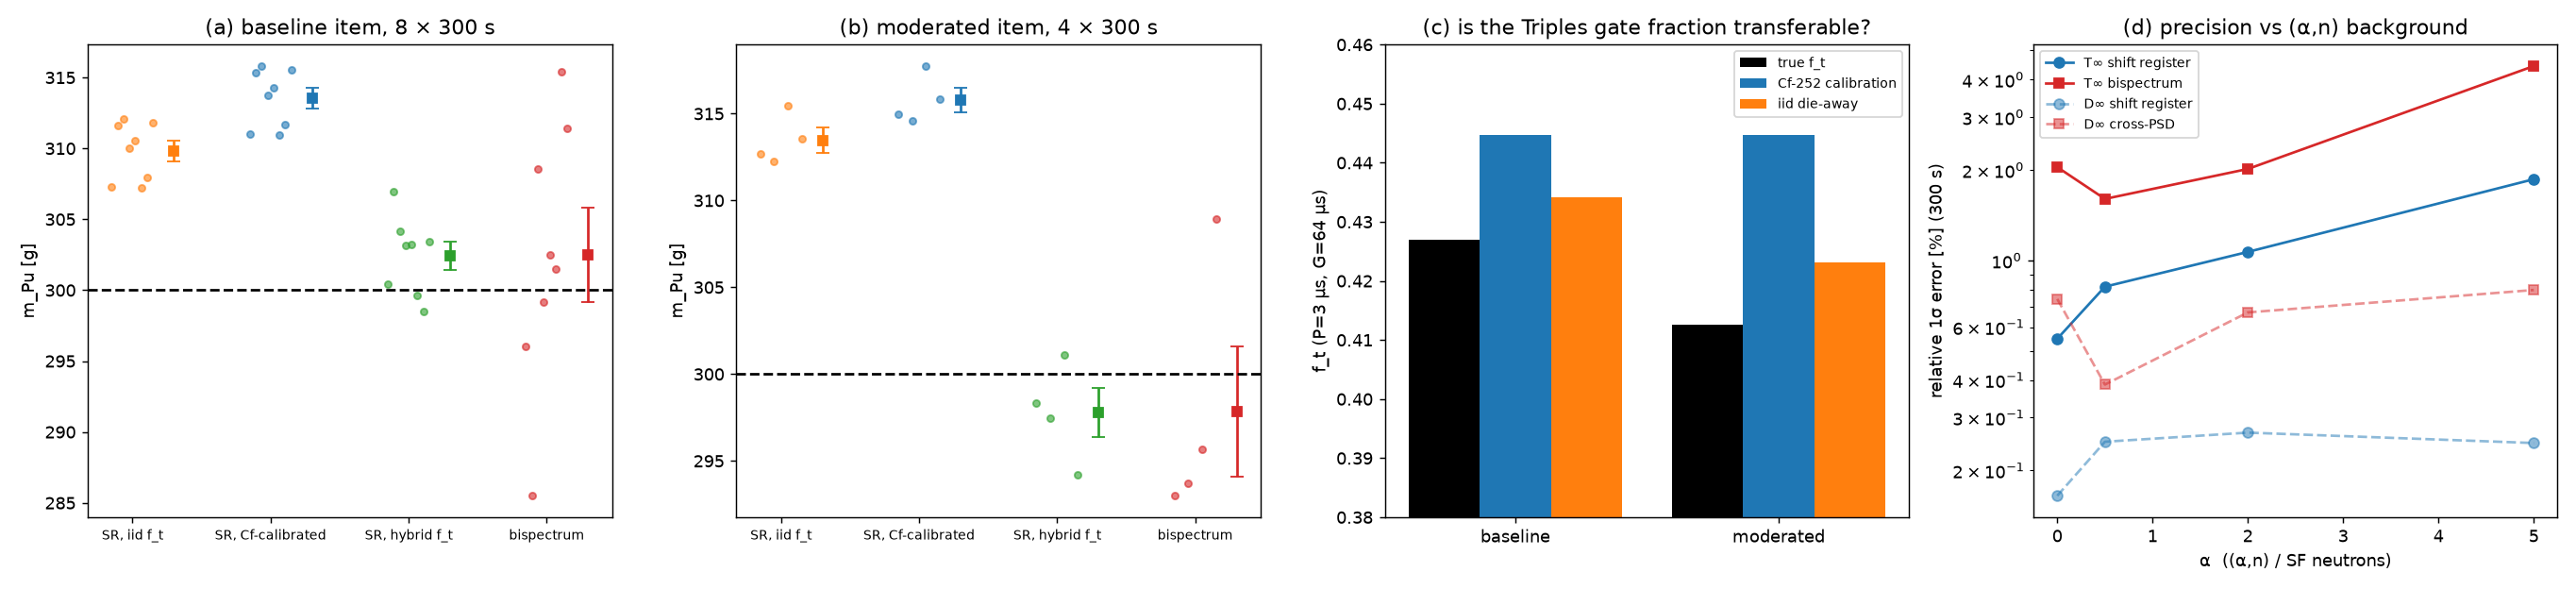
\includegraphics[width=\linewidth]{step_06_studies.png}
\caption{(a, b) Mass per run (dots) and mean $\pm$ standard error (squares) for four
estimators, baseline and moderated item. (c) Triples gate fraction: the true value
($T/\Tinf$) compared with the Cf-252 calibration and the iid die-away estimate. (d) Relative
1$\sigma$ error of $\Dinf$ and $\Tinf$ against the $(\alpha,n)$ ratio, from the in-run
block errors; these overestimate the bispectrum error by about $1.5\times$ (Study A).}
\label{fig:studies}
\end{figure}

\begin{table}[h]
\centering\small
\begin{tabular}{@{}llcccc@{}}
\toprule
Item & Method & mean $m_{\text{Pu}}$ (g) & bias & spread / run (g) & RMS error (g) \\
\midrule
Baseline  & SR, iid $f_t$            & 309.8 & $+3.3\%$ & 2.1 & 10.0 \\
(8 runs)  & SR, Cf-252 calibrated    & 313.5 & $+4.5\%$ & 2.1 & 13.7 \\
          & Bispectrum               & 302.5 & $+0.8\pm1.1\%$ & 9.5 & 9.2 \\
          & \textbf{Hybrid}          & 302.4 & $+0.8\pm0.3\%$ & 2.8 & \textbf{3.5} \\
\midrule
Moderated & SR, iid $f_t$            & 313.5 & $+4.5\%$ & 1.4 & 13.5 \\
(4 runs)  & SR, Cf-252 calibrated    & 315.8 & $+5.3\%$ & 1.4 & 15.8 \\
          & Bispectrum               & 297.8 & $-0.7\pm1.3\%$ & 7.5 & 6.8 \\
          & \textbf{Hybrid}          & 297.8 & $-0.7\pm0.5\%$ & 2.8 & \textbf{3.3} \\
\bottomrule
\end{tabular}
\caption{Study results (300\,s runs, true mass 300\,g). RMS error $=\sqrt{\langle(m-300)^2\rangle}$ combines bias and spread.}
\label{tab:studies}
\end{table}

\paragraph{What the studies show.}
\begin{enumerate}
  \item \textbf{The gate fraction does not transfer} (Fig.~\ref{fig:studies}c). Cf-252 gives
        $f_t=0.445$, while the true values are 0.427 (baseline) and 0.413 (moderated). A Cf
        fission is a single burst. A Pu item adds chain timing: neutrons return from the
        moderator and cause delayed fissions in Pu-239, which spreads the triplets in time,
        and a polyethylene shell makes this stronger. Triples are therefore underestimated by
        4\% and 7\%. This is the classic matrix effect. The calibration source cannot see it,
        but the bispectrum measures it directly.
  \item \textbf{The bispectrum is unbiased on both items}: $\Tinf$ is $-0.6\%$ from truth in
        both cases, with a real spread of 1.9\% per run. The block-error estimate used in
        Table~\ref{tab:res} ($\pm3.8\%$) was pessimistic.
  \item \textbf{On total error for a single measurement, the bispectrum already beats the
        calibrated shift register}: RMS 9.2 against 13.7\,g, and 6.8 against 15.8\,g for the
        moderated item.
  \item \textbf{The hybrid is best}: shift-register precision without the bias, RMS about 3\,g
        on both items. It needs a set of measurements of the same item type to calibrate
        $f_t$ (here 7 other runs, about 35\,min). No calibration source is required.
  \item \textbf{No high-rate advantage} (Fig.~\ref{fig:studies}d). The bispectrum stays 2--4
        times less precise on $\Tinf$ across $\alpha=0$--5. Its noise grows with the
        Singles rate at least as fast as the shift-register cross-term does.
\end{enumerate}

\paragraph{Caveat.} The size of the chain-timing effect depends on how often neutrons
return to the item and fission. OpenMC gets the mean fission rates right but treats fission
implicitly, so the exact $f_t$ shift in a real item may differ. The direction of the effect
is physical: real Pu items do multiply returned thermal neutrons. It should be checked with
an analog multiplicity code (e.g.\ MCNPX-PoliMi) or with measurements.

%==========================================================================
\section{Conclusions}
%==========================================================================
\begin{itemize}
  \item \textbf{Shift register (legacy):} precise ($\approx2$\,g per 300\,s run) but
        \emph{biased} by its Triples gate fraction $f_t$. Calibrating $f_t$ with Cf-252, as a
        real counter does, makes the bias \emph{worse} ($+4.5\%$, and $+5.3\%$ for a moderated
        item), because a Cf source has no fission-chain timing.
  \item \textbf{Cross-PSD and cross-bispectrum (new):} \emph{unbiased} on both items, with
        no gate fractions and no calibration source. Its rates are read at zero frequency,
        where the die-away response equals one, and the background cancels by construction.
        It costs precision: about 9\,g per 300\,s run, 2--4 times worse on $\Tinf$, with no
        gain at high $(\alpha,n)$ rates.
  \item \textbf{The case for the bispectrum} is \emph{accuracy without calibration}, most of
        all for items whose matrix changes the chain timing. Even alone, its total error for a
        single measurement is smaller than that of a Cf-calibrated shift register.
  \item \textbf{Recommended use:} the \textbf{hybrid}. The bispectrum measures $f_t$ for the
        item type, and the shift register delivers the precision. This gives about 3\,g RMS
        on 300\,g (1\%).
  \item \textbf{Next steps:} confirm the chain-timing effect with an analog fission code or
        with measurements; improve the bispectrum precision (frequency weighting, constrained
        kernel); test a single-measurement hybrid.
  \item \textbf{Model limitation:} OpenMC fixed-source fission is implicit. The absolute
        induced-fission moments are effective values, but all methods analyse the same pulse
        trains, so the comparison is valid.
\end{itemize}

\paragraph{Reproducibility.} All code is in \texttt{pu\_multiplicity\_spectral/}, organised
as one folder per step (00--06), each with a smoke test, logs and plots. The geometry figures
are made by \nolinkurl{documentation/make_geometry_figures.py}.

\end{document}
